\begin{frame}[allowframebreaks]{Autoencoders: Architecture}
\begin{figure}
    \centering
    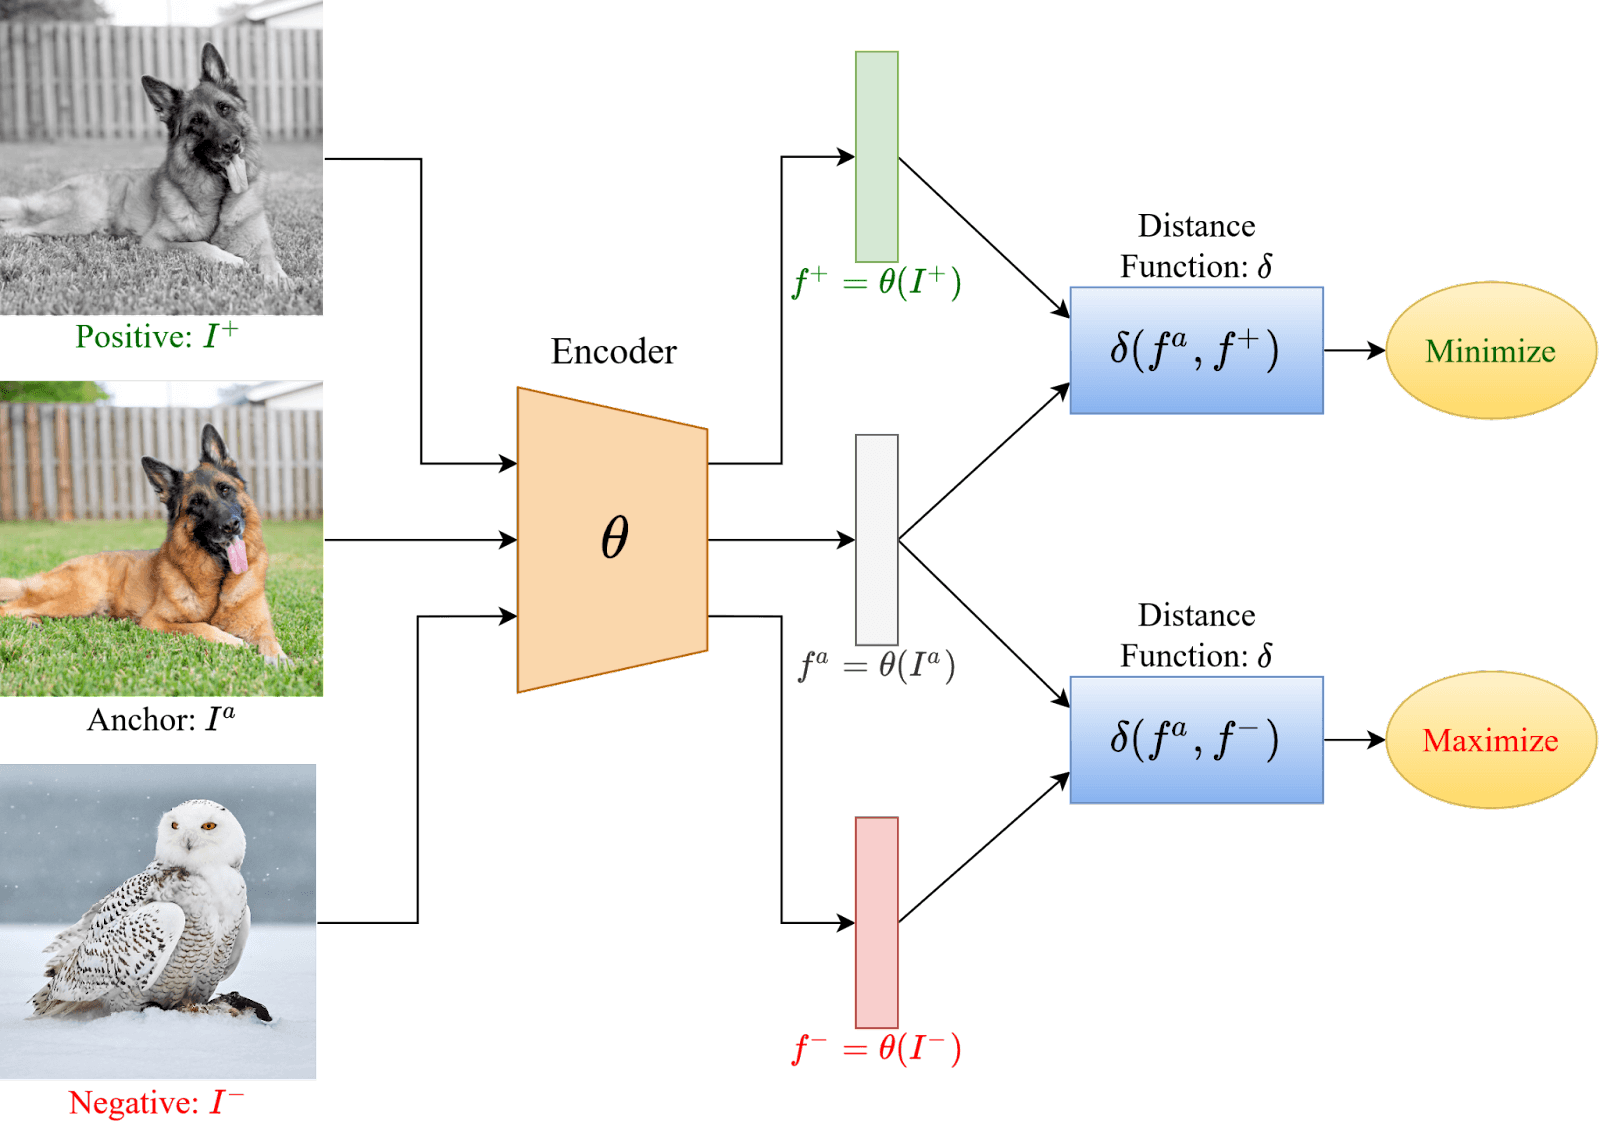
\includegraphics[height=0.9\textheight, width=\textwidth, keepaspectratio]{images/autoencoder/architecture.png}
    \caption{Autoencoder architecture}
\end{figure}

\framebreak

\textbf{Design Considerations}:
\small
\begin{itemize}
    \item \textbf{Depth}: Deeper architectures can capture more abstract representations but may increase the risk of overfitting and require more training data.
    \item \textbf{Width}: Wider layers (more neurons) increase model capacity but can reduce compression effectiveness.
    \item \textbf{Symmetry}: Encoders and decoders are often symmetrical but do not have to be. Asymmetrical designs may be better suited for specific tasks.
    \item \textbf{Regularization}: Techniques such as dropout, weight decay (L1/L2), and sparsity constraints help reduce overfitting and improve generalization.
    \item \textbf{Latent Dimension Size}: A crucial parameter that determines how compressed the representation is. Too small may lose information; too large may not compress enough.
    \item \textbf{Activation Functions}: Nonlinearities like ReLU, sigmoid, or tanh allow the model to learn complex mappings. The final layer typically uses a sigmoid or linear activation depending on the output format.
\end{itemize}
\normalsize

\begin{table}[h!]
\centering
\begin{tabular}{|>{\raggedright\arraybackslash}m{2cm}|>{\raggedright\arraybackslash}m{8cm}|}
\hline
\textbf{Component} & \textbf{Description} \\
\hline
Encoder & Transforms the input data into a compressed latent representation using layers such as Dense, Convolutional, or Recurrent layers. \\
\hline
Latent Space (Bottleneck) & The central compact representation of the input. Forces the model to learn the most essential features. \\
\hline
Decoder & Reconstructs the input from the latent space. Typically mirrors the encoder’s structure in reverse. \\
\hline
Loss Function & Measures the difference between input and output (e.g., Mean Squared Error, Binary Cross-Entropy). Drives learning during training. \\
\hline
Training & Involves minimizing reconstruction error using gradient-based optimization methods such as SGD or Adam. \\
\hline
\end{tabular}
\caption{Architecture Summary Table}
\end{table}

\framebreak

\begin{figure}
    \centering
    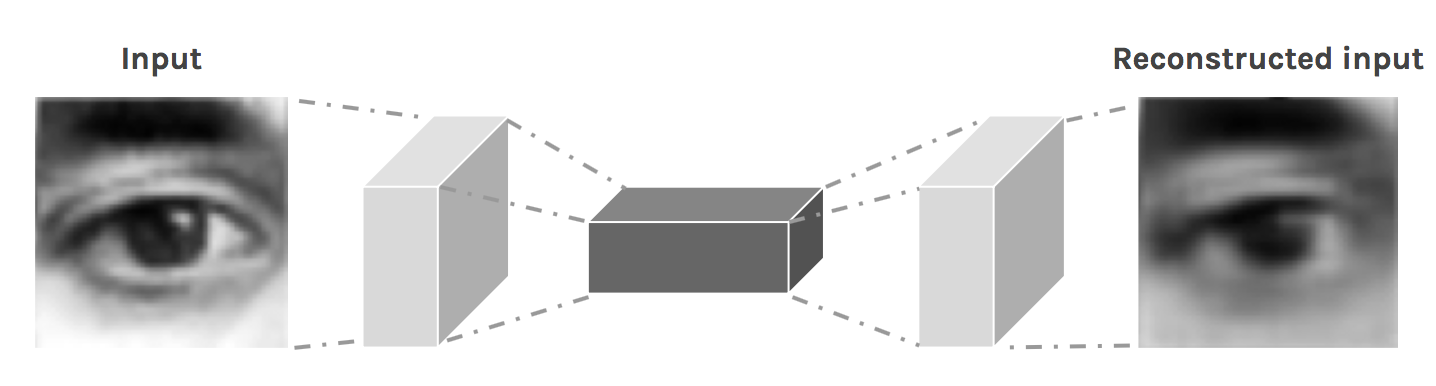
\includegraphics[height=0.9\textheight, width=\textwidth, keepaspectratio]{images/autoencoder/sample.png}
    \caption{Sample Autoencoder}
\end{figure}
\end{frame}

\begin{frame}{Autoencoders: Interactive Demo}
    \centering
    \href{https://douglasduhaime.com/posts/visualizing-latent-spaces.html}{https://douglasduhaime.com/posts/visualizing-latent-spaces.html}
\end{frame}